\section{Results and Discussion}
\label{sec:results}
% \begin{figure}
% \centering
% 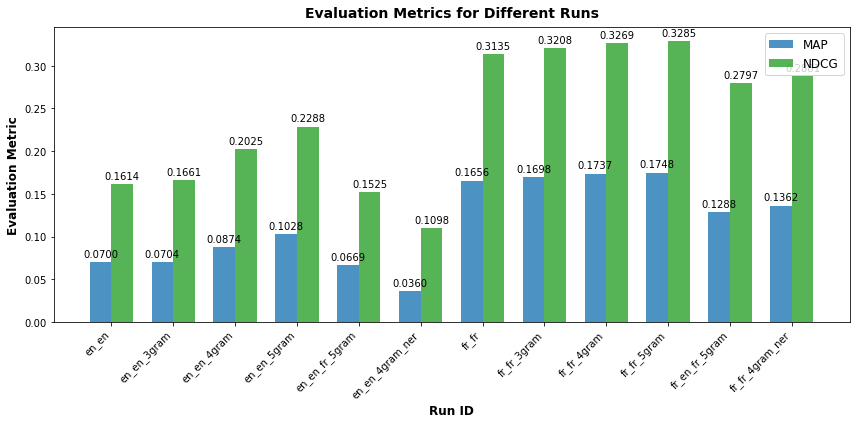
\includegraphics[width=1\textwidth]{figure/chart.png}
% \end{figure}

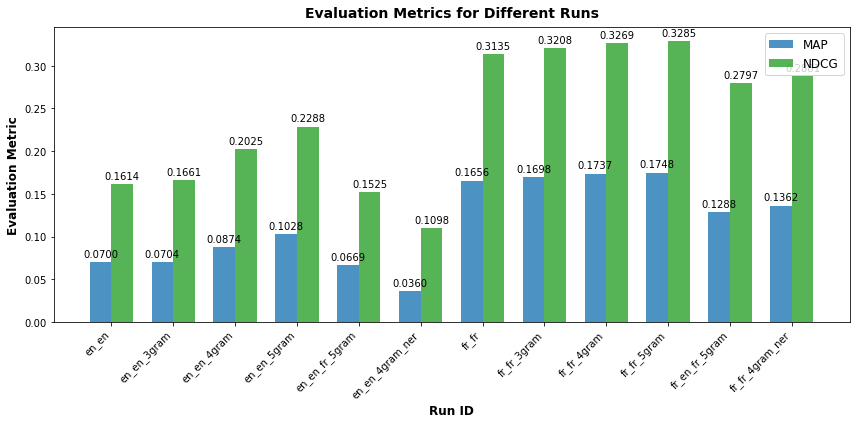
\includegraphics[width=1\textwidth]{figure/chart.png}

The dataset comprises MAP and NDCG scores for twelve
runs of an Information Retrieval (IR) system with different
language models and n-gram sizes for indexing. MAP measures how
effectively the IR system returns relevant results for a given
query, while NDCG indicates the ranking quality of the results.\\

The analysis shows that the highest MAP score (0.1028) is achieved by en\_en\_5gram", 
followed by fr\_fr\_5gram" (0.1748) and fr\_fr\_4gram" (0.1737), while the lowest MAP score (0.0360) is obtained by en\_en\_4gram\_ner". Similarly,
the highest NDCG score (0.3208) belongs to fr\_fr\_4gram\_ner", followed by fr\_fr\_5gram" (0.3285) and
 fr\_fr\_4gram" (0.3269), whereas the lowest NDCG score (0.1098) corresponds to en\_en\_4gram\_ner".\\

The results suggest that French queries perform better than their
English counterparts, possibly due to the training data's origin in
French and later translation into English. Moreover, the IR system's
effectiveness generally increases with a larger n-gram size, as indicated
by the higher scores of en\_en\_5gram" and fr\_fr\_5gram". Conversely, the
inclusion of named entity recognition (ner) in the indexing process seems
to have a negative impact on the scores, as shown by the lower scores of
en\_en\_4gram\_ner" and fr\_fr\_4gram\_ner".\\






